\definecolor{dkgreen}{rgb}{0,0.6,0}
\definecolor{gray}{rgb}{0.5,0.5,0.5}
\definecolor{mauve}{rgb}{0.58,0,0.82}
\definecolor{backcolour}{rgb}{0.95,0.95,0.92}

\lstset{frame=none,
backgroundcolor=\color{backcolour}, 
  language=Python,
  aboveskip=5mm,
  belowskip=5mm,
  showstringspaces=false,
  columns=flexible,
  basicstyle={\linespread{0.8}\small\ttfamily},
  numbers=none,
  numberstyle=\tiny\color{gray},
  keywordstyle=\color{dkgreen},
  commentstyle=\color{blue},
  stringstyle=\color{mauve},
  breaklines=false,
  breakatwhitespace=true,
  tabsize=3
}

\chapter{Application for Image Augmentation}

\section{Image Augmentation Background}

Convolutional Neural Networks (CNNs) have quickly become a go-to solution for image classification following the popularization of deep learning \cite{dataAugment}. CNNs start with an input representation of an image such as the a 3D matrix of RGB values. With a convolution step, a tile is slid across the input and applies filters on each region to compute new features and store them in an output feature map. The CNN continues to learn by finding values for the filter matrix that can better extract useful features from the input feature map. In a pooling step, the feature map is downsampled while preserving its critical features. This means that with each new layer in the network, the dimensions of the input are reduced while expanding the depth of the feature map. The end result is one or more fully connected layers where every node in a higher level layer is connected to every node in the lower level layer. A final output function can use the final layer to compute the probability that the input image matches a given classification.

\quad One common problem with these networks, however, is overfitting. Overfitting refers to a phenomena where the model created starts to closely match the input training data. This is a problem if the input data set does not generalize well to a variety of other valid inputs. The first most obvious solution to this problem is to make sure input data sets are sufficiently large and varied. This is a problem, however, in applications such as medical imaging where there aren't enough inputs available to overcome overfitting \cite{imageAugmentationSurvey}. Data augmentation refers to another possible solution to this problem where a smaller input data set is augmented with a series of transforms and modifications to produces a larger output set \cite{dataAugment, effectivenessDataAugmentation}. 

\quad Many tools exist for this such as the Python deep learning library Keras that includes whats called an \verb|ImageDataGenerator| \cite{keras}. This class allows users to construct an object instance using a variety of parameters that are used to generate augmented output images. Using the \verb|ImageDataGenerator| class, images are produced in real-time as they are needed by the training model. Python image augmentation libraries conventionally perform the augmentation itself on the CPU while performing the learning itself on the GPU. This creates a unique opportunity to use the constructs included in Millipyde to create an on-device augmentation function similar to Keras' \verb|ImageDataGenerator|.

\section{Image Augmentation in Millipyde}

In addition to having accessible CPU counterparts for comparison, there are many other advantages to experimenting with image augmentation in Millipyde. Since image augmentation is based on image transformations, it is ripe for GPU accelerations, and it can leverage Millipyde's builtin \verb|gpuimage| methods. The results were also easy to verify. Initial implementations used probabilities of 1 for guaranteed function execution as well as single-point ranges for each random image transformations. Millipyde's testing scripts could then verify with pixel-level accuracy that each image matched the expected output. The probability could gradually be lowered in addition to introducing larger random ranges to introduce higher degrees of variability into the results. Each \verb|gpuimage| can be manually inspected for verification, and multiple were used to confirm that there was a degree of random variation. 

\quad As shown in the sample code in Figure \ref{augmentCode}, the Millipyde code can closely mirror the behavior of other image augmentation libraries. By choosing the Generator rather than the Pipeline, results can be produced on the fly as they are needed by a future training model. The Generator's copy semantics also lets us produce an output set that is larger than the original input set. For the purpose of this demonstration, the \verb|return_to_host| flag was set to true and the images were saved as output files that can be viewed and studied. In practice, it may be desirable to avoid saving the images entirely and to keep their memory contents on-device so that it can be used by the learning-phase. This demo resulted in 48 new images created from an input size of 6 images as shown in Figure \ref{augmentResults}. 

\begin{figure}
\begin{lstlisting}
from skimage.io import imsave

import millipyde as mp

def augment():
    images = mp.images_from_path("examples/augment_in")

    ops = [
        mp.Operation("transpose", probability=.2),
        mp.Operation("fliplr", probability=.2),
        mp.Operation("random_brightness", -.2, 1),
        mp.Operation("random_gaussian", 0, 2),
        mp.Operation("random_colorize", [.5, 1.5], [.5, 1.5], [.5, 1.5], 
                probability=.3),
        mp.Operation("rgb2grey", probability=.3),
        mp.Operation("random_rotate", 0, 120, probability = .5)
    ]

    g = mp.Generator(images, ops, return_to_host=True)

    for i in range(48):
        img = next(g)
        imsave("examples/augment_out/dog" + str(i) + ".png", img)
    
def main():
    augment()

if __name__ == '__main__':
    main()
\end{lstlisting}
\caption{The Python code used to augment images using Millipyde.}
\label{augmentCode}
\end{figure}

\begin{figure}[hbtp]
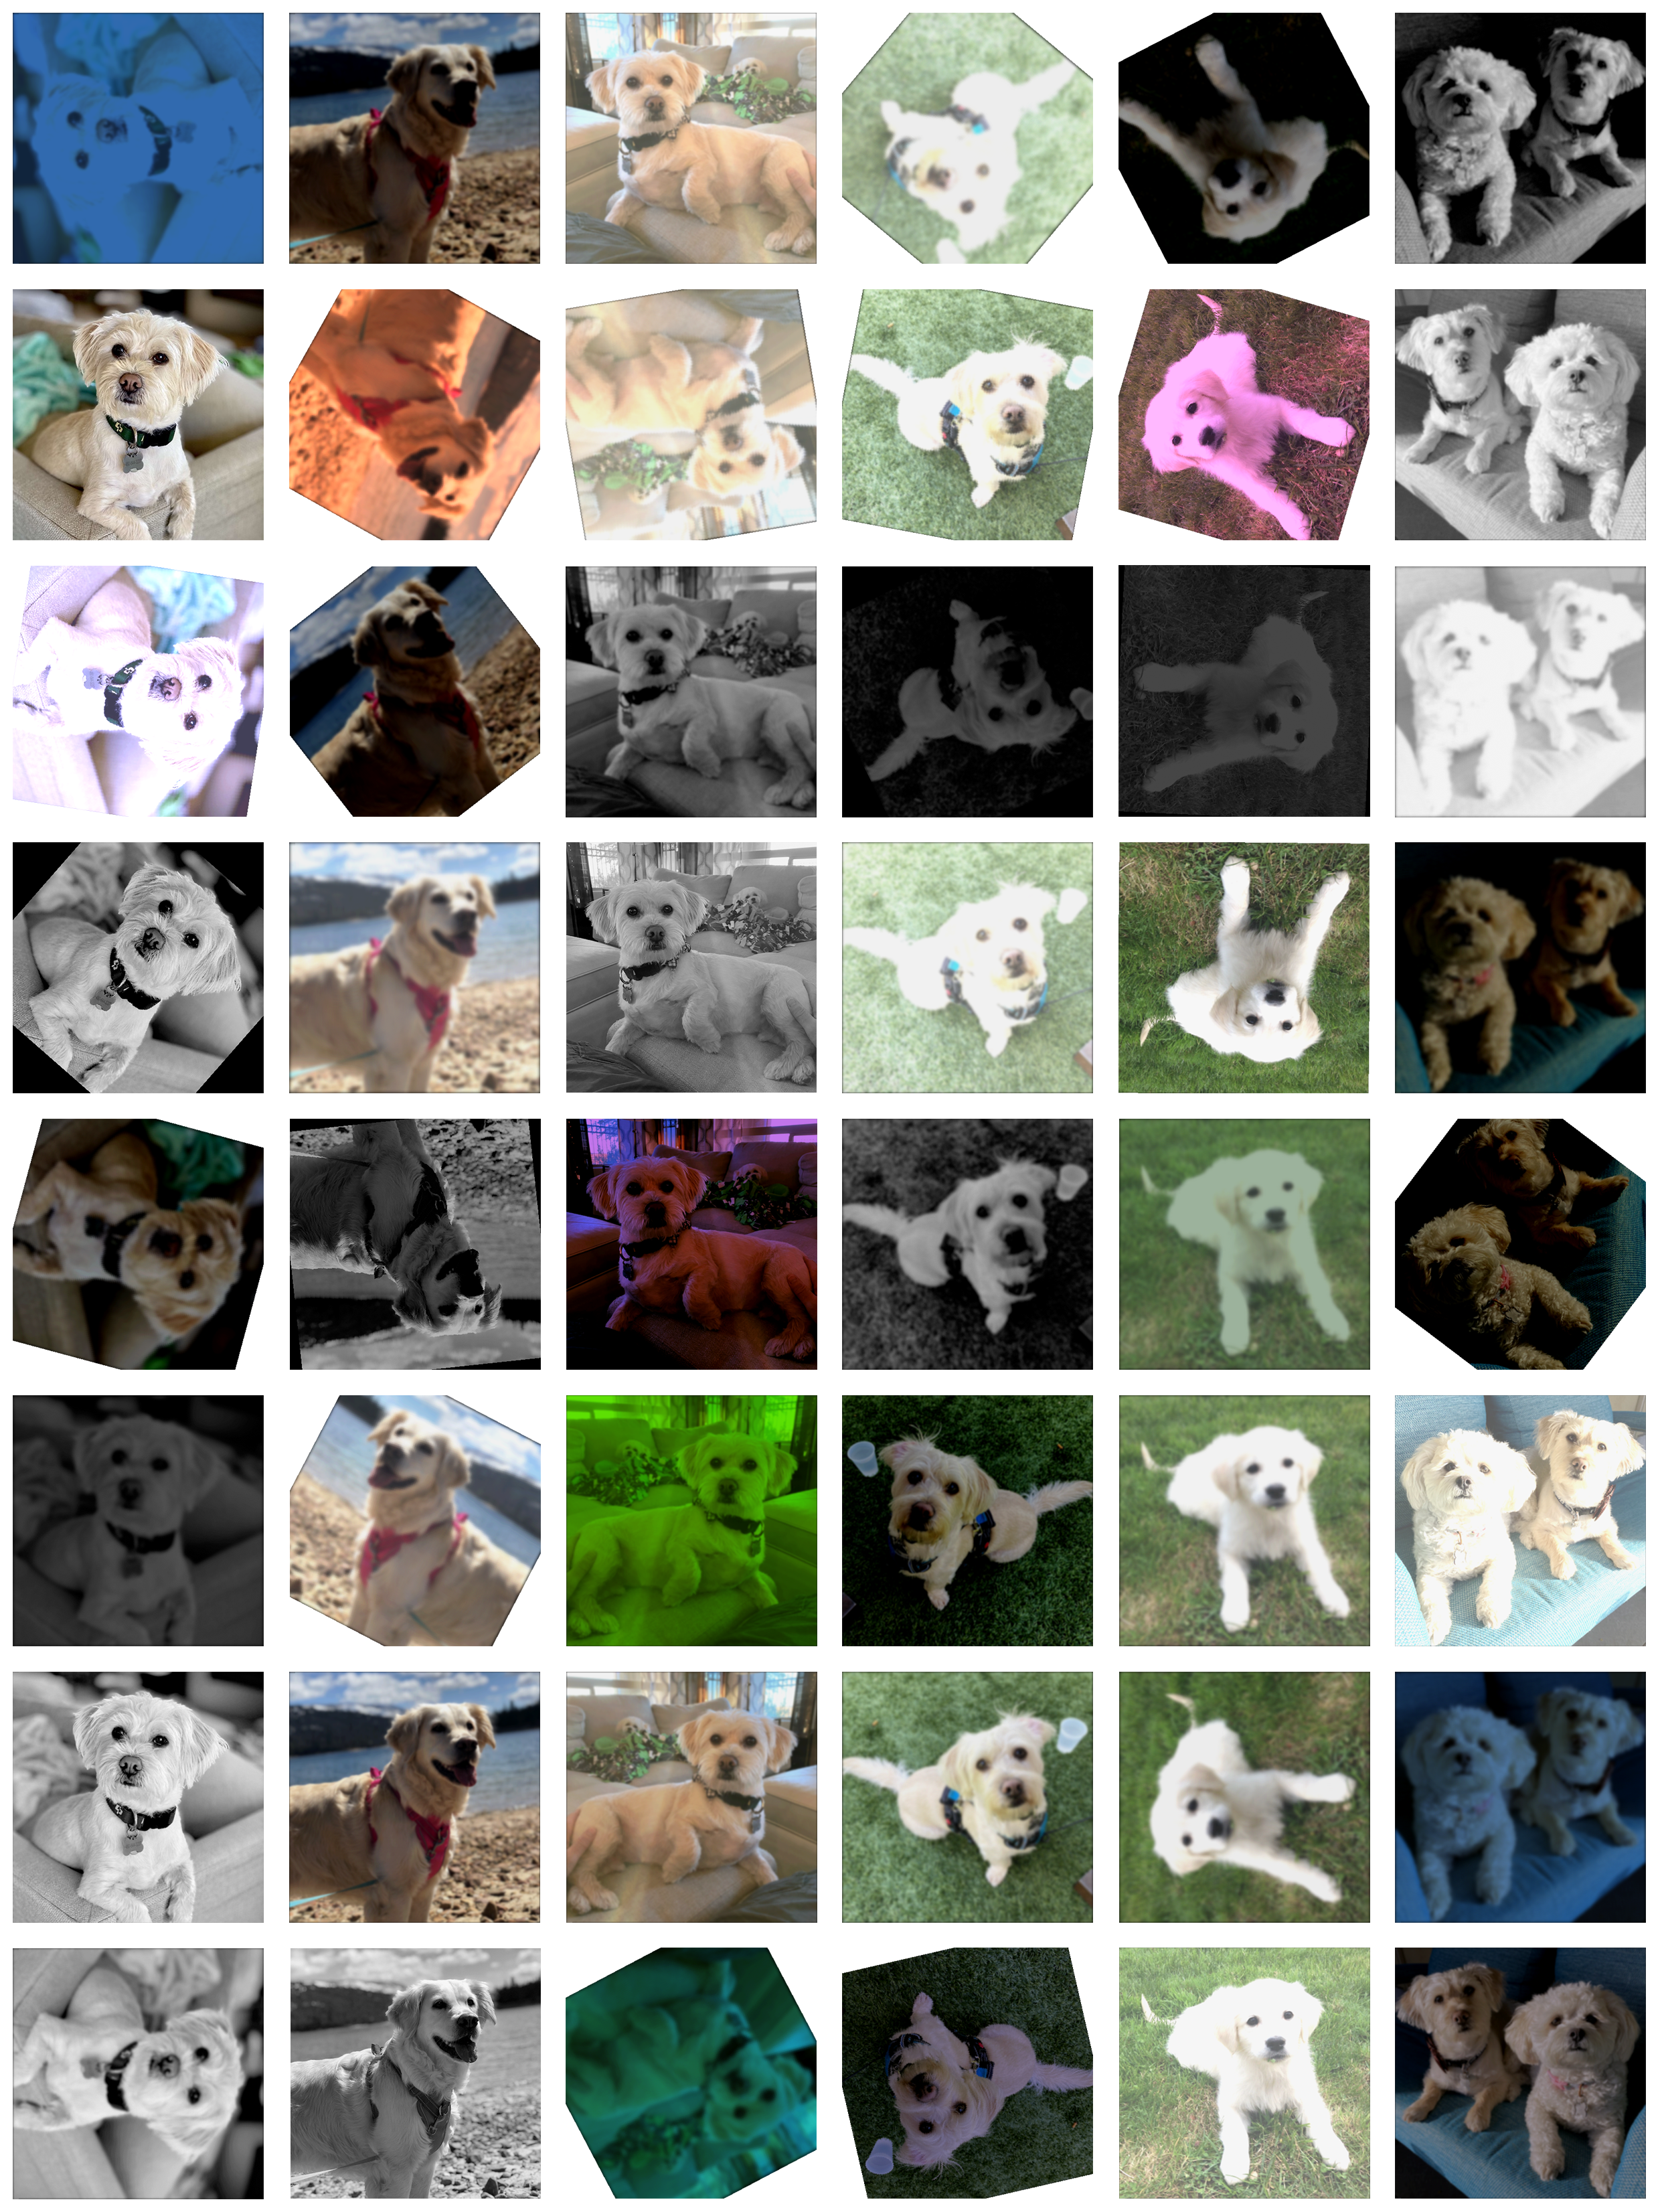
\includegraphics[width=\textwidth]{figures/AugmentationResults.png}
\centering
\caption{Augmenting six input images to produce 48 output images}
\label{augmentResults}
\end{figure}

\section{Results Discussion}

Each column in Figure \ref{augmentResults} represents an augmentation of one of the same six original input images. As seen in the diversity across each row, our implementation succeeded in producing a wide variety of results. No two images ended up quite the same, but each output could be used as an example of a dog for a future training algorithm. In some cases, the transformations might be too extreme to work optimally for image classification applications, so the parameters and probabilities can be further tuned by users in this field. The dog in the first image, for example, loses some of its edges to the background with the combination of random transformations selected. We look forward to testing Millipyde augmentation in-depth with future practical computer vision applications.